\documentclass[nobib]{tufte-handout}

%\\geometry{showframe}% for debugging purposes -- displays the margins

\newcommand{\bra}[1]{\left(#1\right)}
\usepackage{hyperref}
\usepackage[activate={true,nocompatibility},final,tracking=true,kerning=true,spacing=true,factor=1100,stretch=10,shrink=10]{microtype}
\usepackage{color}

% Fixes captions and images being cut off
\usepackage{marginfix}

\usepackage{pgfplots}
\usepackage[americancurrents, americaninductors, americanvoltages, americanresistors]{circuitikz}
\usepackage{siunitx}
\usepackage{amsmath,amsthm}
\usetikzlibrary{shapes}
\usetikzlibrary{positioning}
\usetikzlibrary{arrows}

% Set up the images/graphics package
\usepackage{graphicx}
\setkeys{Gin}{width=\linewidth,totalheight=\textheight,keepaspectratio}
\graphicspath{{.}}

\title{Notes for ECE 30500 - Semiconductor Devices}
\author[Shubham Saluja Kumar Agarwal]{Shubham Saluja Kumar Agarwal}
\date{\today}  % if the \date{} command is left out, the current date will be used

% The following package makes prettier tables.  We're all about the bling!
\usepackage{booktabs}

% The fancyvrb package lets us customize the formatting of verbatim
% environments.  We use a slightly smaller font.
\usepackage{fancyvrb}
\fvset{fontsize=\normalsize}

% Small sections of multiple columns
\usepackage{multicol}
\usepackage{mdframed}

% These commands are used to pretty-print LaTeX commands
\newcommand{\doccmd}[1]{\texttt{\textbackslash#1}}% command name -- adds backslash automatically
\newcommand{\docopt}[1]{\ensuremath{\langle}\textrm{\textit{#1}}\ensuremath{\rangle}}% optional command argument
\newcommand{\docarg}[1]{\textrm{\textit{#1}}}% (required) command argument
\newenvironment{docspec}{\begin{quote}\noindent}{\end{quote}}% command specification environment
\newcommand{\docenv}[1]{\textsf{#1}}% environment name
\newcommand{\docpkg}[1]{\texttt{#1}}% package name
\newcommand{\doccls}[1]{\texttt{#1}}% document class name
\newcommand{\docclsopt}[1]{\texttt{#1}}% document class option name

\newmdenv[
    backgroundcolor=black!10, % Light blue shading inside the box
    linecolor=black,         % Border color
    linewidth=1pt,          % Border thickness
    roundcorner=5pt,        % Rounded corners
    skipabove=10pt,         % Space above the box
    skipbelow=10pt,         % Space below the box
    innertopmargin=5pt,     % Inner top margin
    innerbottommargin=5pt,  % Inner bottom margin
    innerleftmargin=10pt,   % Inner left margin
    innerrightmargin=10pt   % Inner right margin
    ]{defbox}

\newmdenv[
    backgroundcolor=cyan!10, % Light blue shading inside the box
    linecolor=cyan,         % Border color
    linewidth=1pt,          % Border thickness
    roundcorner=5pt,        % Rounded corners
    skipabove=10pt,         % Space above the box
    skipbelow=10pt,         % Space below the box
    innertopmargin=5pt,     % Inner top margin
    innerbottommargin=5pt,  % Inner bottom margin
    innerleftmargin=10pt,   % Inner left margin
    innerrightmargin=10pt   % Inner right margin
    ]{notebox}

\newcommand{\defn}[2]{
        \begin{defbox}
        \noindent\textbf{#1}:\ #2
        \end{defbox}
}
\newcommand{\note}[1]{
        \begin{notebox}
        \noindent\textit{Note}:\ #1
        \end{notebox}
}

\begin{document}

\maketitle

\begin{abstract}
    These are lecture notes for Fall 2025 ECE 30500 by professor Haitong Li at Purdue. Modify, use, and distribute as you please.
\end{abstract}

\tableofcontents

\newpage

\section{Properties of Silicon}
The core of semiconductors lies in the silicon transistor. But, why silicon
(\textbf{Si})?\\
\begin{itemize}
    \item Si is the second most common element on Earth.
    \item It is easily purified, and grown defect free, with less than 1 impurity in
          $10^9$ atoms.
    \item Reasonably good electronic properties
    \item Resilient to harsh environments
    \item Excellent mechanical properties
    \item There are three forms of Si: \begin{itemize}
              \item In a Si crystal, atoms are arranged in an orderly array, allowing arrangements
                    to be easily reproduced.
              \item In poly-crystalline Si, many crystalline subsections exist.
              \item In amorphous Si, there are no long range patterns or arrangements.
          \end{itemize}
\end{itemize}
The unit cell is a portion of any crystal that could be used to reproduce the crystal.\\
The primitive cell is the smallest possible unit cell.\\
In essence, a unit cell is a subset of a lattice that can be moved in the x, y, z axis, and cover the entire lattice. (\textit{Note the absence of rotation movements.})\\
Some examples of cells are the following:
\begin{center}
    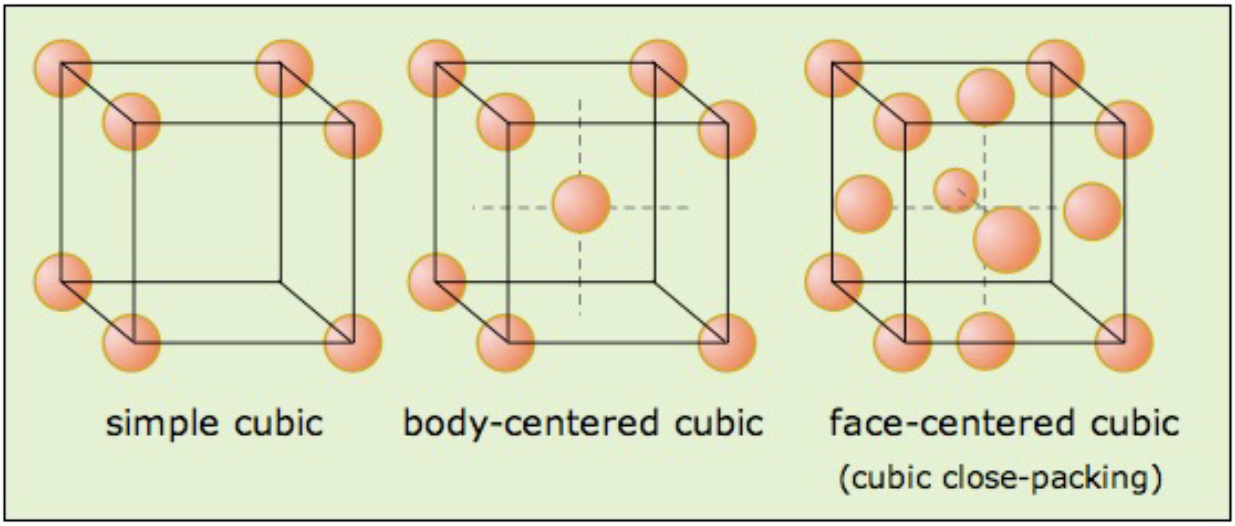
\includegraphics[width = 250px]{images/unit_cell_cube.png}
\end{center}
\note{the image is missing a corner atom.}
Another important cubic unit cell is the diamond cubic unit cell with 8 silicon atoms in the cell:
\begin{center}
    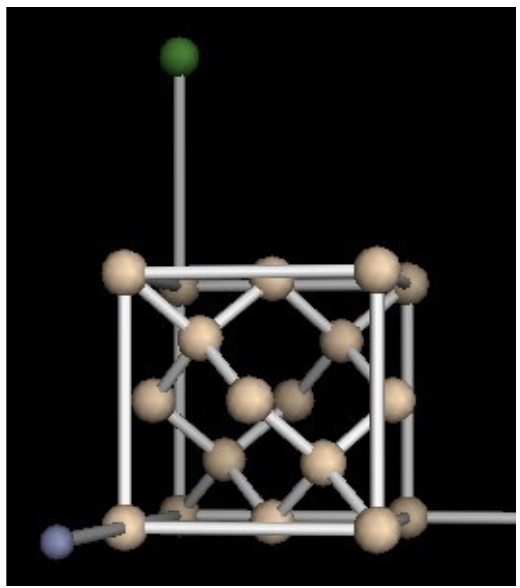
\includegraphics[width = 175px]{images/diamond_cube_cell.png}
\end{center}
\subsection{Density (diamond cube cell)}
Lattice constant: $a=5.3407Ang$\\ Atomic mass: $28.055$amu\\ Density: $\rho =
    \frac{8*28.0855*1.6605*10^{-23}}{(5.4307*10^{-10})^3}kg/m^3 = 2.3296g/cm^3$
\subsection{Miller Indices}
Let us consider a plane that intercepts the axes at $x_{int}, y_{int},
    z_{int}$. The equation of the plane is:
\begin{equation*}
    \frac{x}{x_{int}}+\frac{y}{y_{int}}+\frac{z}{z_{int}} = 1
\end{equation*}
The vector that is perpendicular to this plane will have the same components as the Miller indices.\\
The Miller indices are defined as $LCM*(\frac{1}{x_{int}},\frac{1}{y_{int}},\frac{1}{z_{int}})$.
\section{Energy Bands}
\subsection{Quantization of Energy Levels}
Bohr hypothesized, in his atomic model, that there was a quantization of
electron angular momentum and energy levels.\\ In the context of this class,
these levels will be described by $n \in \mathbb{N}$.\\ Additionally, the
energy of these levels is $E_H = -\frac{13.6}{n^2}eV$.\\ The energy levels of
silicon are as shown below:\\
\begin{center}
    \includegraphics*[height = 100px]{images/si_energy_levels.png}
\end{center}
The further from the core, the more energy is within, so, in the image above, $4S^0$ is the layer with the most energy.\\
The four electrons in the valence region ($3P^2,3S^2$) are the easiest to break away from the atom.
\subsection{Bonding Model}
Only the four valence electrons are of interest. Each of these, is shared with
one of the four nearest neighbors, forming a structure like this:
\begin{center}
    \includegraphics*[width = 100px]{images/silicon_neighbor_bond.png}
\end{center}
This is the base of the silicon lattice, from which more complex lattices can be formed. The full model can be abstracted as follows:
\begin{center}
    \includegraphics*[width = 100px]{images/bonding_model.png}
\end{center}
where a line is a shared valence electron and a circle is the core of the semiconductor.\\
\subsection{Energy Levels}
When going from a single Si atom to a Si crystal with many atoms, the atoms are
closely packed enough that we cannot treat them as individual atoms. The
structure that is formed is very stable as all the atoms and their energy
levels are completely filled.\\ \note{Current cannot flow from full energy
    levels.} The energy levels of these atoms are in the following order:
\begin{eqnarray*}
    &\text{conduction band}\\
    &\cdots \cdots \cdots \\
    &\uparrow \\
    &\text{band gap}\\
    &\uparrow \\
    &\cdots \cdots \cdots \\
    &\text{valence band}
\end{eqnarray*}
The conduction band and the valence band are energy levels where electrons can reside.\\
Electrons can be freed from their bonds by heating the lattice to temperatures close to $300K$. The thermal energy provided by this is defined by:
\begin{equation*}
    E = \frac{3}{2}kT
\end{equation*}
The freed electrons are analyzed in terms of their energy states. When freed, they are moving from the valence band (leaving behind a "hole" in the valence band), jumping over the band gap and arriving at the conduction band.\\
The band representation can be further abstracted to look like this:
\begin{center}
    \includegraphics*[width = 100px]{images/band_diagram_abstraction.png}
\end{center}
Where the red dots are conduction band electrons (n) and the blue dots are valence band holes (p).
\note{an intrinsic semiconductor is that in which $n = p = n_i$.
    \begin{equation*}
        n_i = BT^{\frac{3}{2}}e^{-\frac{E_g}{2k_B T}}
    \end{equation*}
}
\subsection*{Constants to Remember}
\begin{align*}
    E_G(Si)   & = 1.12eV                                        \\
    E_G(GaAs) & = 1.4eV                                         \\
    k_B T     & = 0.026eV \text{ at }(T = 300K)                 \\
    P         & \approx e^{-E_G / k_B T}                        \\
    n_i(Si)   & = 1\times 10^{10} cm^{-3} \text{ at }(T = 300K) \\
    n_i(GaAs) & = 2\times 10^{6} cm^{-3} \text{ at }(T = 300K)  \\
\end{align*}
\subsection*{Material Representations}
\begin{center}
    \includegraphics*[width = 250px]{images/material_representations.png}
\end{center}
Note that the main difference between an insulator and a semiconductor is the size of the band gap. On the other hand, metals have no band gap at all, and all the electrons are free by default.\\
\section{Carrier Properties}
Electrons are in the conduction band, and they can move between states.\\ Holes
are in the valence band, and they can move between states.\\ Electrons and
holes can recombine and regenerate.\\ \textbf{When there are no perturbing
    forces, equilibrium occurs.}\\ When a highly energetic photon hits an electron
in the valence band, it pushes it into the conduction band and leaves a hole
behind in the valence band.\\
\begin{equation*}
    E_{ph} = hf \gg E_G
\end{equation*}
Usually, the force on an object is defined by $F = m_0 a$, but, this cannot be so simply applied to the case of forces on electrons. Instead, the formula is:
\begin{equation*}
    F = m_n^* a
\end{equation*}
where $m_n^*$ is the effective mass of the electrons, and it includes
\begin{itemize}
    \item Cyclotron
    \item Conductivity
    \item \textbf{Density of States}
\end{itemize}
Similarly, for a hole, $F = m_p^* a$.
\begin{center}
    \begin{tabular}{|c|c|c|}
        \hline
        Materials & $m_n^*/m_0$ & $m_p^*/m_0$ \\
        \hline
        Si        & 1.18        & 0.81        \\
        \hline
        Ge        & 0.55        & 0.36        \\
        \hline
        GaAs      & 0.066       & 0.52        \\
        \hline
    \end{tabular}
\end{center}
The energy of electrons in vacuum resemble a parabola when compared with momentum:
\begin{align*}
    E = \frac{p^2}{2m_0} & \rightarrow E_n = E_C+\frac{p^2}{2m_n^*}             \\
    p = m_0 v            & \rightarrow p = \hbar k = \hbar \frac{2\pi}{\lambda}
\end{align*}
\subsection{Doping}
The following is the process to n-dope a semiconductor sample:
\begin{center}
    \includegraphics*[width = 100px]{images/ndope.png}
\end{center}
and the process for p-doping:
\begin{center}
    \includegraphics*[width = 100px]{images/pdope.png}
\end{center}
\begin{itemize}
    \item N-doping: When n-doping, with group V elements, very little energy is necessary
          to break the fifth electron from the element.\\ The ionized donor is then left
          with 4 electrons and is bound to the lattice.\\ The energy band diagram looks
          like the following:
          \begin{center}
              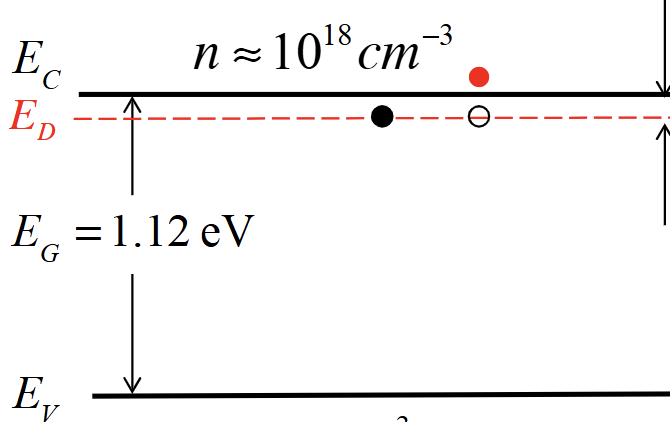
\includegraphics[height = 100px]{images/energy_bond_doping.png}
          \end{center}
          The released donor electron joins the conduction band. This is easy due to how close $E_D$ and $E_C$ are.
    \item P-doping: Similar to n-doping, except, that it is with holes instead of
          electrons. Thus, the band diagram looks like this:
          \begin{center}
              \includegraphics*[height = 100px]{images/energy_p_doping.png}
          \end{center}
          Once again, very little energy is necessary for the transition (accepting, in this case) to occur.
\end{itemize}
This whole process has a dependance on temperature, with higher temperatures providing more energy to the elements, and thus facilitating the bonding process.\\
\subsection{Density of State (DOS)}
\defn{Density of States ($g(E)$)}{Number of states per unit of energy per unit volume.}
There are $4N_a \frac{states}{band}$ where $N_a = 5\times 10^{22}/cm^3$.\\
$g(E)dE$ is the number of states in an energy range.
Energy states are distributed as follows:
\begin{center}
    \includegraphics*[height = 150px]{images/dos.png}
\end{center}
And, based on the above equation:
\begin{equation*}
    \int_{E_c^{top}}^{E_c} g_C(E)dE = 4N_a = \int_{E_V}^{E_V^{bot}} g_V(E)dE
\end{equation*}
which leads to some very complicated expressions which are later approximated using:
\begin{equation*}
    E = \frac{\hbar^2k^2}{2m^*}
\end{equation*}
\subsection{Fermi Level and Function}
The following is the Fermi function:
\begin{equation*}
    f(E) = \frac{1}{1+e^{(E-E_F)/k_B T}}
\end{equation*}
where $k_B = 8.617\times 10^{-5} eV/K$ is the Boltzmann Constant.\\
The Fermi function defines the probability of an electron energy state being filled at a given temperature within an atom in equilibrium.
\note{$f(E_f) = \frac{1}{2}$ because it is the very border, so it behaves as a step function, with 1 below and 0 above.}
The Fermi Level ($F_E$) is the top of the energy levels electrons would have if they were at $T=0K$. This is because, electrons cannot occupy the same energy level, and thus, at absolute zero, they pack themselves together at the lowest available energy levels, thus filling up all the levels beneath the Fermi Level.
It can move up and down based on the compositionn of the material, being affected by things like doping.\\
Looking at the Fermi function allows us to notice the temperature dependance of the probability, with probabilties of high energies increasing with higher temperatures.\\~\\
In an intrinsic semiconductor, the Fermi level is exactly between the conduction and valence bands, making the fermi function probabilties have the following property: $f(E_C) = 1-f(E_V)$.
\subsection{Carrier Distributions}
\end{document}
